\section{Packet Reception Rate}
\label{sec:packet_reception_rate}

The effect of temperature and other environmental factors on link quality has most thoroughly been investigated with the conclusion that all measurements of link quality deteriorate with higher temperature, as one would expect~\cite{Wennerstrom2013, Boano2013, Boano2014, Zuniga2013}.
However, Boano~\etal{} showed in their experiments that this behavior is not symmetrical, since heating the transmitter caused a more significant drop in \ac{PRR} than heating the receiver~\cite{Boano2013}.

In this experiment we used the same physical setup as described in Section~\ref{subsec:effects_of_temperature}, but with random payload as message content.
We fixed mote rotation to create a link that is just starting to deteriorate at \SI{50}{\celsius}, so that at low temperatures the link is of good quality, while at very high temperatures the link will experience high \ac{BER}s.

We increased the temperature of the mote in box 0 in steps of \SI{5}{\celsius} and \SI{10}{\celsius} up to \SI{80}{\celsius} and kept the mote on box 1 at constant \SI{30}{\celsius}, while sending 180.000 messages back and forth.
Then we repeated this, but heated box 1 and kept box 0 temperature constant.
To cancel out environmental factors we ran this experiment four times over two days, so we could then pick the two results with the least interference.

For the evaluation we plotted the normalized \ac{PRR} of messages sent from one mote and received by the other mote over temperature and time and included \ac{BER} and \ac{LQI} and \ac{RSSI} values to illustrate link quality.
Figure~\ref{fig:prr_link_01} shows messages sent from mote 0 addressed to mote 1 for both temperature cycles, while Figure~\ref{fig:prr_link_10} shows the opposite direction.
It becomes immediately clear that a higher temperature of either transmitter or receiver makes the link quality worse, validating the findings of Boano~\etal{} and Wennerstr{\"o}m~\etal~\cite{Boano2013, Wennerstrom2013}.
However, this relationship is neither linear nor symmetrical.


\subsection{Effects of Temperature on \acs{PRR} and \acs{BER}}

In Figure~\ref{fig:prr_link_01} the decrease in \ac{PRR} is small and relatively symmetrical up to about \SI{65}{\celsius}, however, past that point we see a dramatic change, with the increments in temperature translating very strongly into significant drops in \ac{PRR}.
The drop in \ac{PRR} is not symmetrical and becomes much more pronounced, when the receiver is heated than when the transmitter is heated, especially visible in the last increment from \SI{70}{\celsius} to \SI{80}{\celsius}.

This asymmetry is even more extreme in link 1-0, shown in Figure~\ref{fig:prr_link_10}, where heating the receiver beyond \SI{70}{\celsius} will cause an almost complete loss of message reception.
Interesting is the little dip in \ac{PRR} around \SI{50}{\celsius} in Figure~\ref{fig:prr_link_10_receiver}, which was present in this link in all four experiments with varying intensity. We suspect that this is a non-linearity in the radio, cases of which have also been reported by Boano~\etal

The \ac{BER} acts like an inverse function of \ac{PRR}, since higher \ac{BER} yields more messages with at least one bit error.
Noise on \ac{PRR} is visible in the standard deviation of \ac{BER} as exemplified by Figure~\ref{fig:prr_link_10_transmitter}.


\subsection{Effects of Temperature on \acs{LQI} and \acs{RSSI}}

The \ac{LQI} is a very good mirror of the \ac{PRR} of messages without error.
When the receiver is kept at a constant temperature, the values decrease almost linearly with temperature of the transmitter.
This is not the case when the receiver is heated, where a linear correlation to temperature , but is still very similar to the behavior of \ac{PRR}.
We therefore can confirm that \ac{LQI} is a good source for an estimate on \ac{PRR}.

This is very much not the case with \ac{RSSI}, which has much lower resolution that \ac{LQI} and exhibits hysteresis and non-linearities~\cite{Boano2013}.
While in Figure~\ref{fig:prr_link_01}, \ac{RSSI} ends up being lower when the receiver is heated than when it is constant, Figure~\ref{fig:prr_link_10} shows very similar values, even though \ac{PRR} is radically different.

It is also noteworthy that contrary to \ac{LQI}, \ac{RSSI} attempts to describe signal strength (\ie the power level being received by the antenna), which of course does not change, when the transmitter is at constant temperature.
Therefore, without temperature information, the \ac{RSSI} value is misleading, since it represents the power level not at the antenna, but at the signal amplifying stage of the radio. 
Therefore \ac{RSSI} is usable for a very inaccurate estimate of link quality at best, with little to no difference between receiver and transmitter temperature.


\subsection{Discussion}

Our data strongly implicates the receiver as being more vulnerable than the transmitter to an increase in temperature, especially above \SI{65}{\celsius}.
These results are very much incompatible with the findings of Boano~\etal~\cite{Boano2013}, which is surprising since the only two differences between our experiment and theirs is the temperature range and the additional usage of the CC2520~\cite{cc2520} radio, which is very similar to the CC2420~\cite{cc2420}.
However, these differences should not account for completely opposing results.

Research by Bannister~\etal~\cite{Bannister2008} saw an asymmetry in output and received input power when heating transmitter and receiver separately.
At the same time, they measured \ac{PER} and found that above \SI{-90}{\dBm} \ac{RSSI}, temperature had little to no influence, while below that \ac{RSSI} value, \ac{PER} increased.
The authors concluded that the CC2420 \acl{LNA} stage is less efficient at high temperature, which would manifest itself in a significant increase in \ac{PER} (or a \emph{decrease} in error-free \ac{PRR}) on the receiver.
However, the \ac{RSSI} behavior in Figure~\ref{fig:prr_link_10} does not reflect a general truth of the results by Bannister~\etal{} and furthermore suggests no direct correlation between \ac{RSSI} and \ac{PRR}.

We noticed a strong focus in such research on understanding the impact of temperature on output and input signal power, however, it seems that \ac{RSSI} does not actually correspond to link quality in general.
From our data, a combination of \ac{LQI} and temperature seems to have the best correlation to \ac{PRR}, therefore we want to examine how we can use temperature to improve \ac{PRR} in these conditions.

\begin{figure}[t]
	\subfigure[Constant receiver, increasing \newline transmitter temperature.] {
		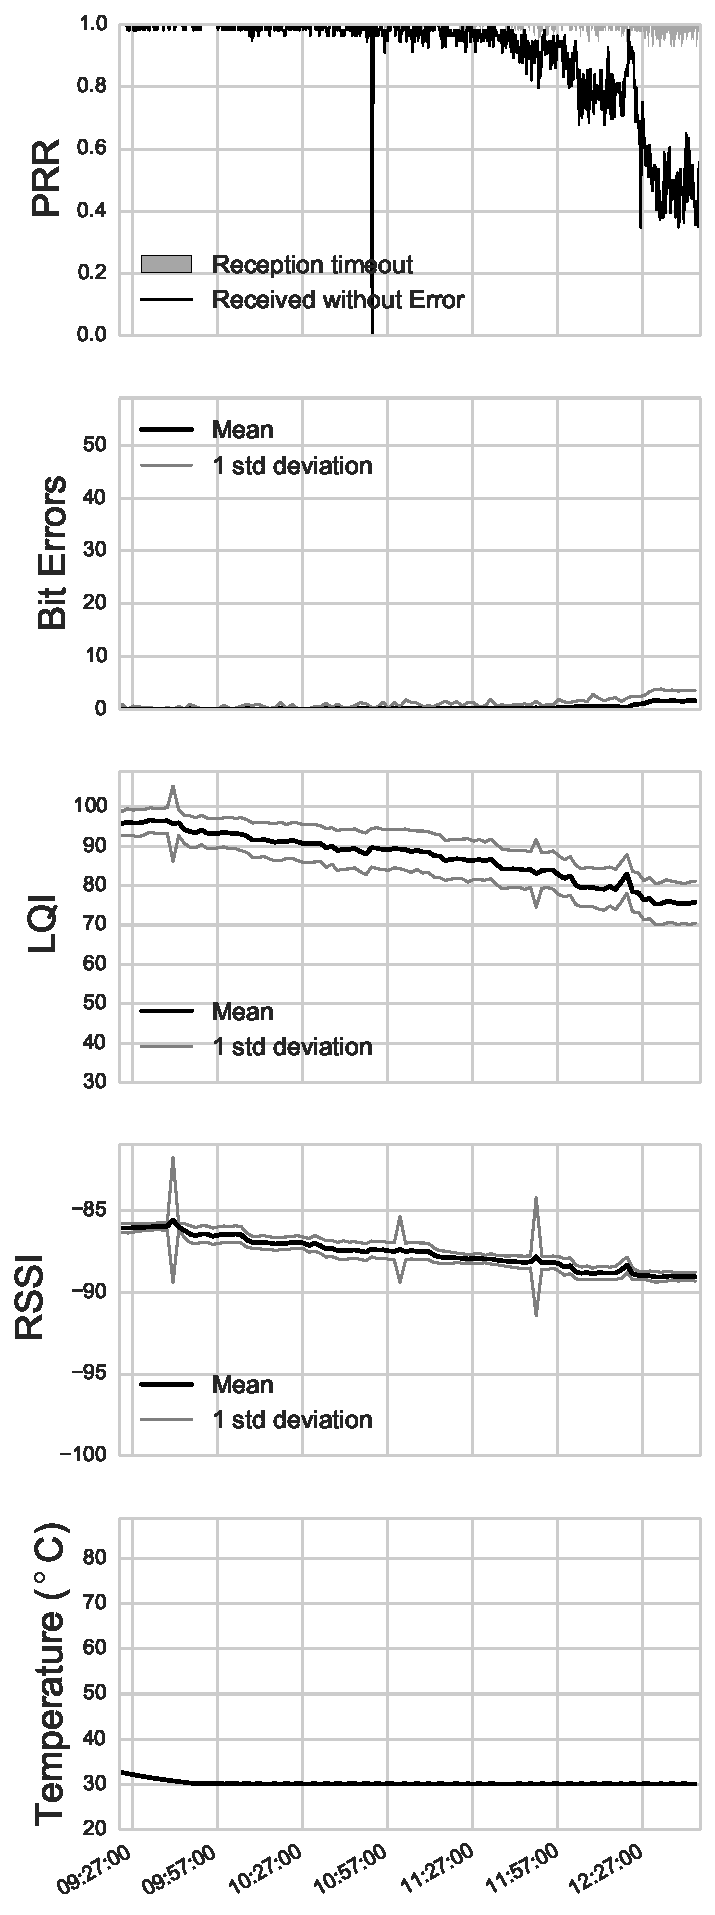
\includegraphics[width=0.475\columnwidth]{figures/prr_0-1_transmitter}
		\label{fig:prr_link_01_transmitter}
	}
	\subfigure[Increasing receiver, constant \newline transmitter temperature.] {
		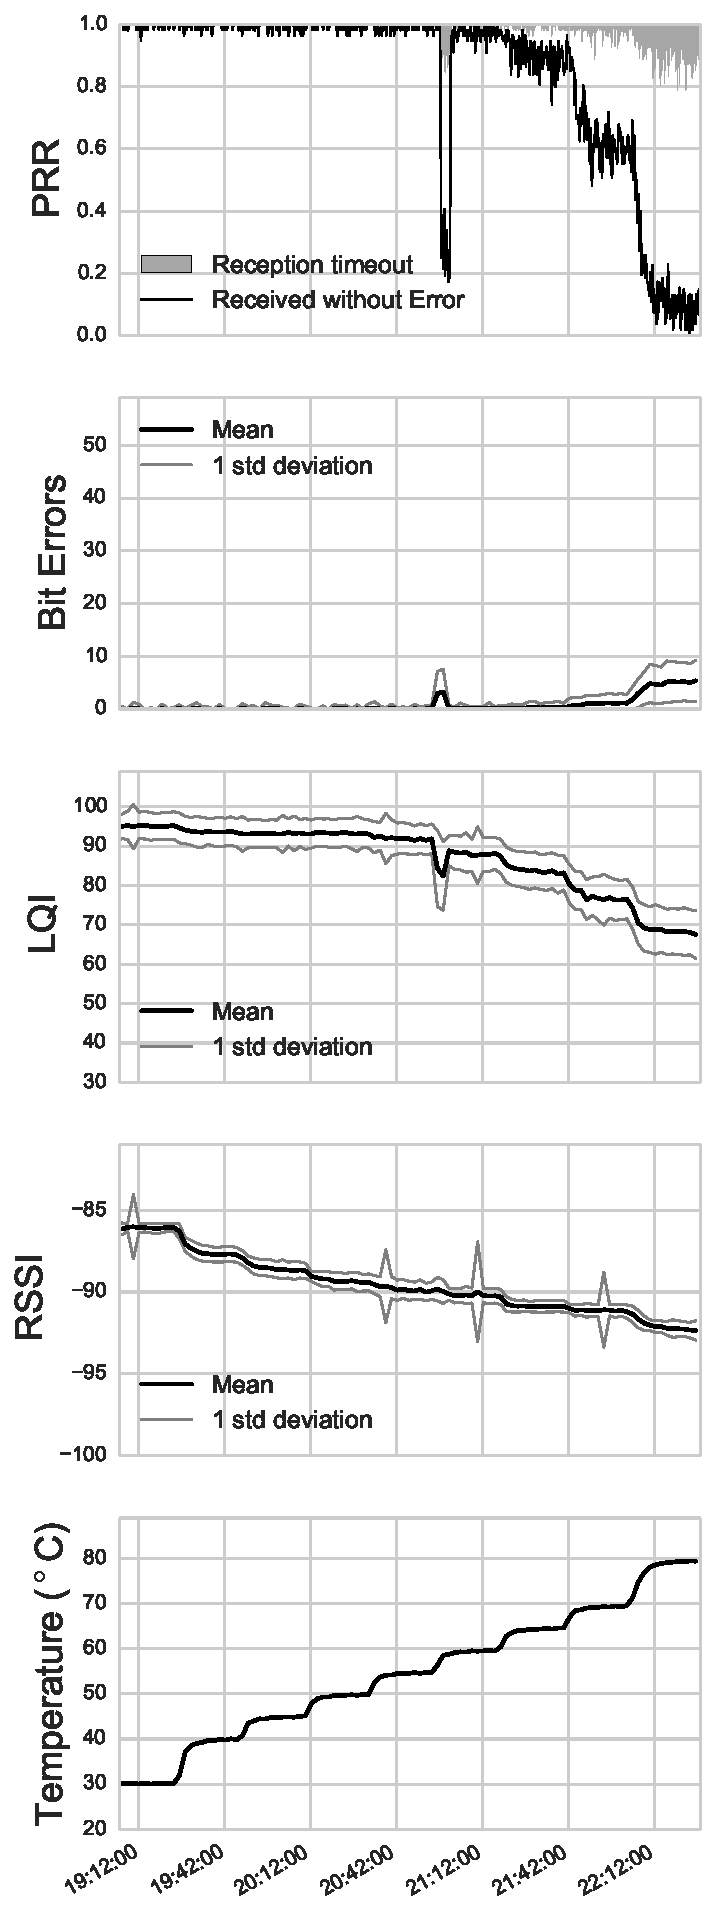
\includegraphics[width=0.475\columnwidth]{figures/prr_0-1_receiver}
		\label{fig:prr_link_01_receiver}
	}
	\caption{\acs{PRR} and link quality of messages received by mote \textbf{1} vs. temperature. For transmitter temperature see Figure~\ref{fig:prr_link_10}.}
	\label{fig:prr_link_01}
\end{figure}

\begin{figure}[t]
	\subfigure[Increasing receiver, constant \newline transmitter temperature.] {
		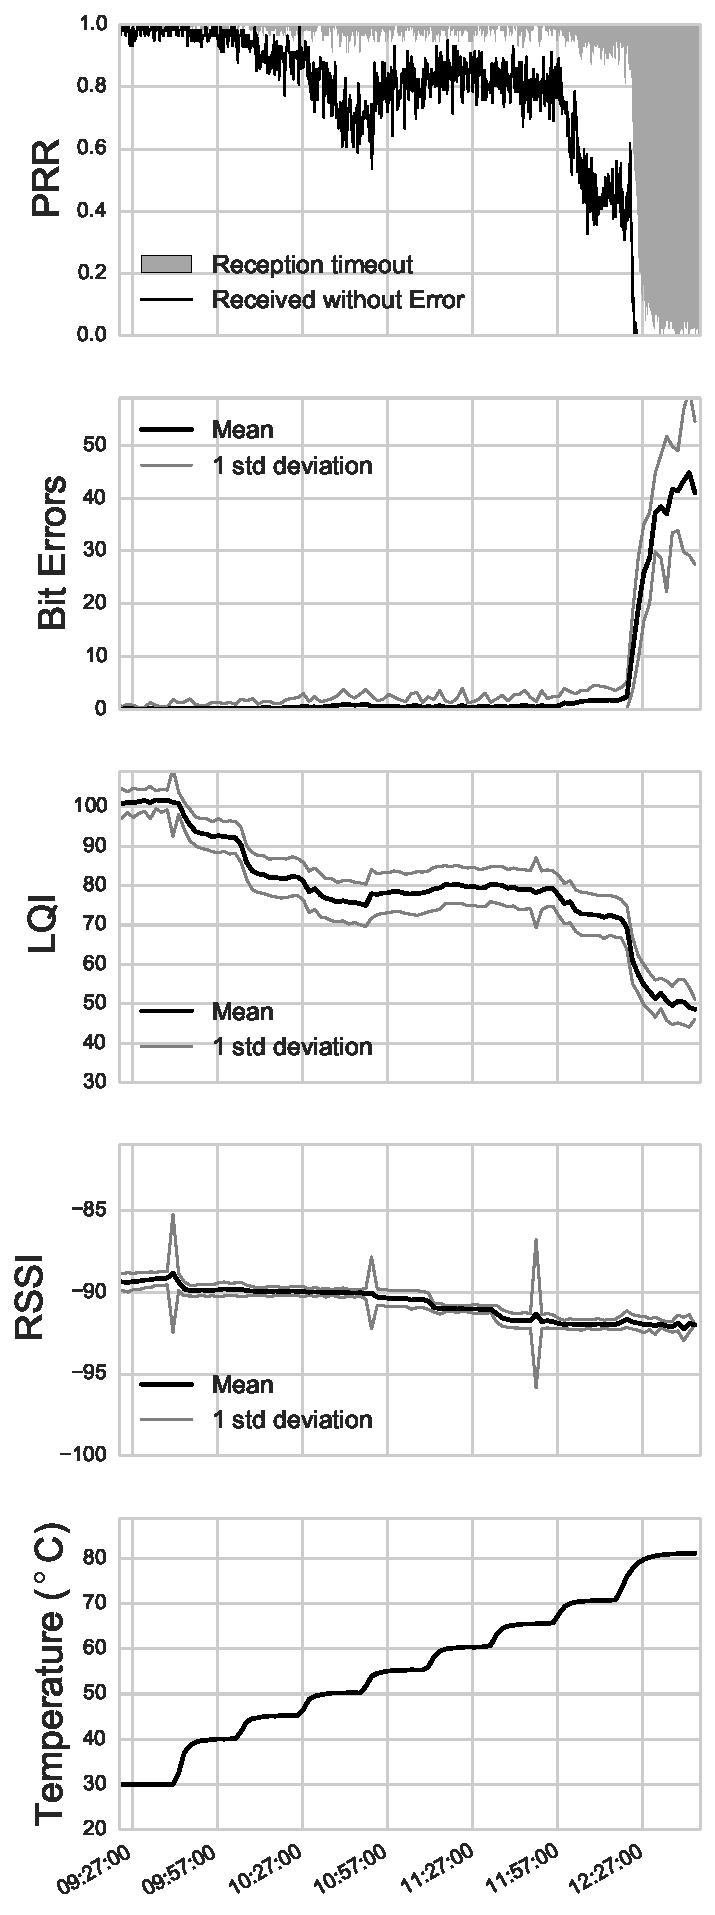
\includegraphics[width=0.475\columnwidth]{figures/prr_1-0_receiver}
		\label{fig:prr_link_10_receiver}
	}
	\subfigure[Constant receiver, increasing \newline transmitter temperature.] {
		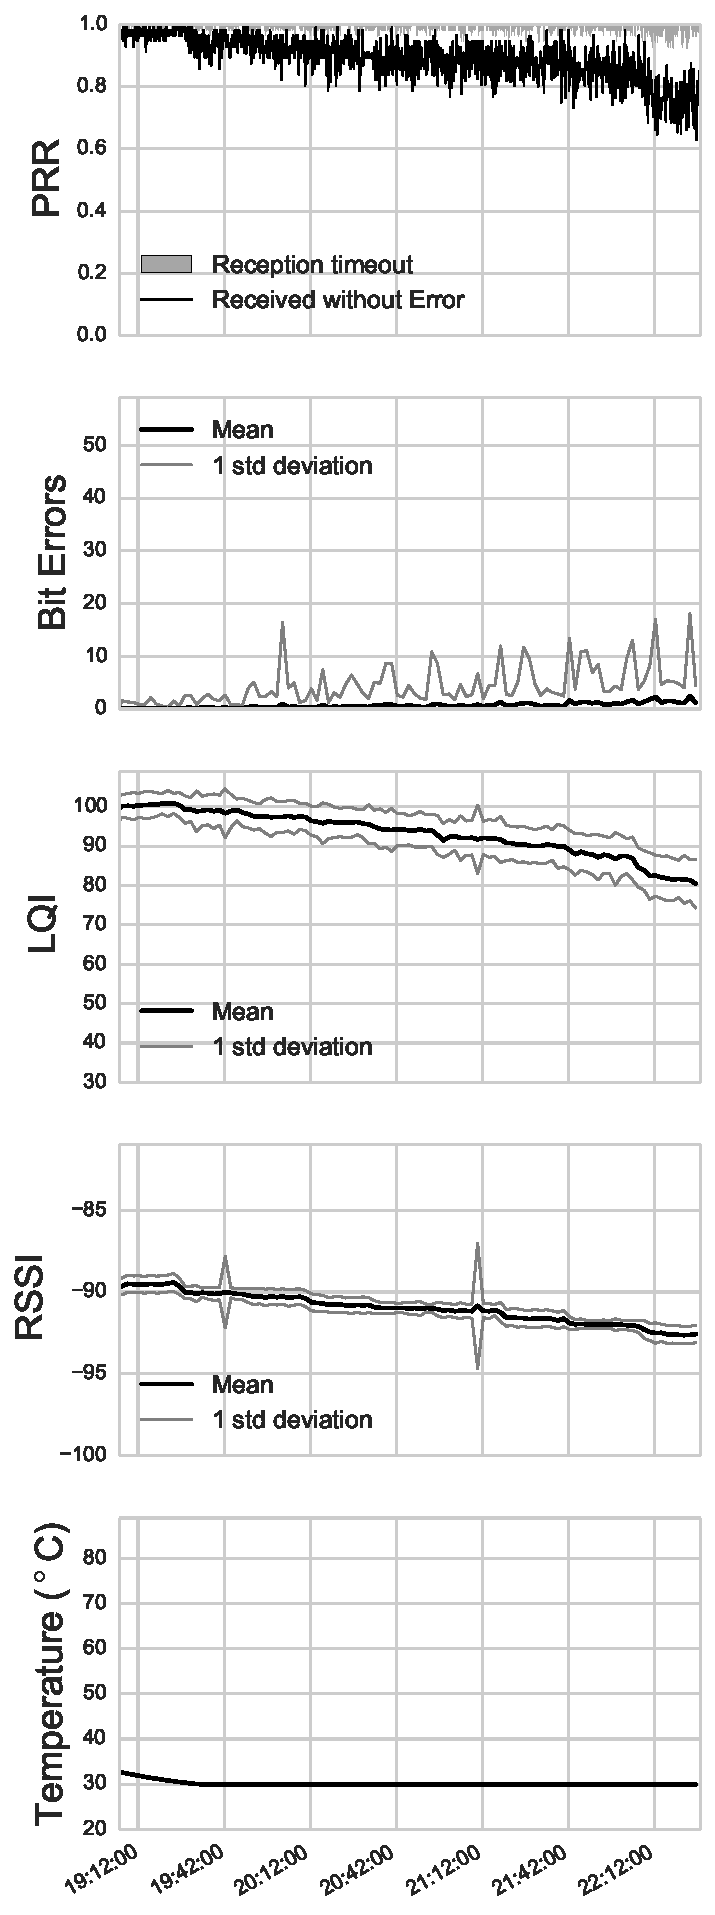
\includegraphics[width=0.475\columnwidth]{figures/prr_1-0_transmitter}
		\label{fig:prr_link_10_transmitter}
	}
	\caption{\acs{PRR} and link quality of messages received by mote \textbf{0} vs. temperature.  For transmitter temperature see Figure~\ref{fig:prr_link_01}. The asymmetry in \acs{PRR} shows much more clearly here.}
	\label{fig:prr_link_10}
\end{figure}

